\chapter{Spectres électroniques et magnétisme des complexes}\label{ch:b3:complex-spectra-magnetism}

Le rubis est rouge et l'émeraude verte, et pourtant tous deux doivent leur
couleur au même ion, \ce{Cr^{3+}}, qui remplace quelques ions aluminium dans
deux oxydes différents~: le corindon,
$\ce{Al2O3}$, pour le rubis, et le béryl, un silicate d'aluminium et de
béryllium, pour l'émeraude. Dans les deux, le chrome occupe un octaèdre
d'atomes d'oxygène~; dans le béryl, l'octaèdre est un peu plus grand et le
champ des ligands un peu plus faible, et les bandes d'absorption de l'ion se
déplacent d'environ un millier de nombres d'onde vers le rouge. Cela suffit à
faire passer la couleur transmise du rouge au vert. Ce chapitre explique
quantitativement de tels spectres~: comment les termes d'un ion libre se
scindent dans un champ des ligands, comment les \omterm{def:b3:complex-spectra-magnetism:tanabe-sugano}{diagrammes de
Tanabe--Sugano} transforment les positions de deux bandes en éclatement du
champ des ligands et en répulsion électronique, pourquoi certaines bandes
sont intenses et d'autres faibles, pourquoi certains complexes se
déforment, et comment le magnétisme compte les électrons non appariés.

\begin{recall}
Le volume de deuxième année a traité des éléments de transition et de leurs
configurations $d^n$, de l'éclatement du champ cristallin $\Delta_{\mathrm o}$, des complexes
haut spin et bas spin, de l'énergie d'appariement, de l'énergie de
stabilisation du champ cristallin, des transitions $d$--$d$, de la série
spectrochimique, de la théorie du champ des ligands, et des substances
paramagnétiques et diamagnétiques. Le \cref{ch:b3:many-electron-atoms} a
établi les \omterm{def:b3:many-electron-atoms:term}{symboles de termes} et les règles de Hund, le
\cref{ch:b3:group-theory-applied} la réduction des représentations et les
\omterm{def:b3:group-theory-applied:direct-product}{produits directs}, le \cref{ch:b3:electronic-spectroscopy} a énoncé les
règles de sélection de spin et de Laporte et décrit les \omterm{def:b3:electronic-spectroscopy:charge-transfer}{transitions de
transfert de charge}, et le \cref{ch:b3:partition-functions} a donné la
\omterm{def:b3:partition-functions:boltzmann}{distribution de Boltzmann}.
\end{recall}

\begin{omfigure}
\begin{minipage}[b]{0.3\linewidth}\centering
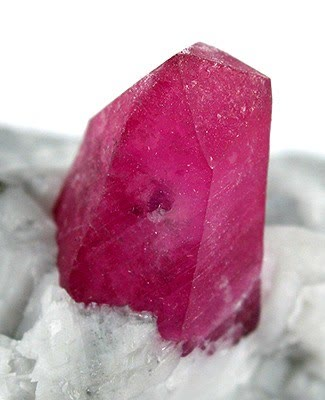
\includegraphics[height=4.2cm]{images/book4/ruby-crystal.jpg}\par
{\small rubis}
\end{minipage}\hspace{1.5em}
\begin{minipage}[b]{0.3\linewidth}\centering
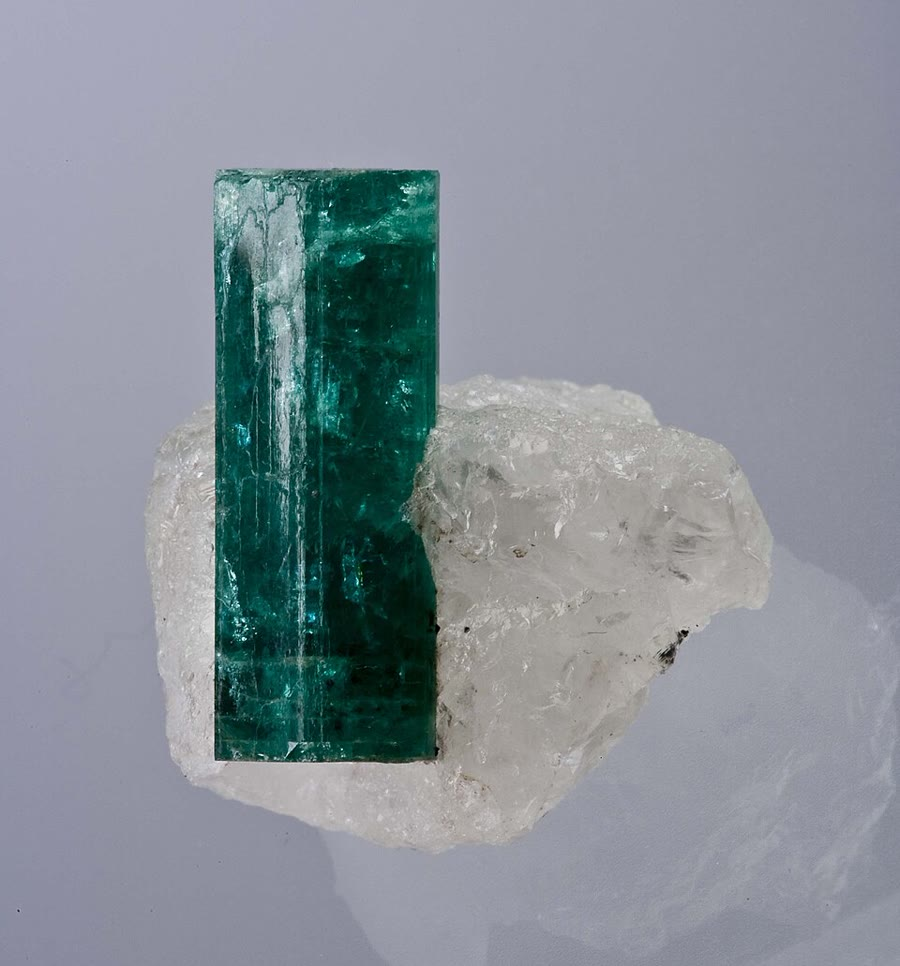
\includegraphics[height=4.2cm]{images/book4/emerald-crystal.jpg}\par
{\small émeraude}
\end{minipage}

{\small Un cristal de rubis dans du marbre et un cristal d'émeraude sur du
quartz. Dans les deux, la couleur vient de quelques pour cent de \ce{Cr^{3+}}
en site octaédrique.}
\end{omfigure}

\section{Des termes de l'ion libre aux termes du champ des ligands}

Dans un ion libre, la répulsion électronique scinde une configuration $d^n$ en
termes ($^4$F, $^4$P, $^2$G\dots\ pour $d^3$, \cref{ch:b3:many-electron-atoms}). Dans un
complexe, chaque terme est de nouveau scindé par les ligands, et les niveaux
sont étiquetés par les \omterm{def:b3:point-groups:irrep}{représentations irréductibles} du \omterm{def:b3:point-groups:point-group}{groupe ponctuel} du
complexe.

\begin{definition}[Terme du champ des ligands]\label{def:b3:complex-spectra-magnetism:ligand-field-term}
Un \emph{terme du champ des ligands}\index{terme du champ des ligands} d'un
complexe est un ensemble d'états polyélectroniques dégénérés, étiquetés par
leur \omterm{def:b3:many-electron-atoms:term}{multiplicité de spin} et par la \omterm{def:b3:point-groups:irrep}{représentation irréductible} du \omterm{def:b3:point-groups:point-group}{groupe
ponctuel} à laquelle appartient leur partie orbitale, comme $^4$A$_{2g}$ ou
$^4$T$_{1g}$ dans un complexe octaédrique.
\end{definition}

\begin{proposition}[Caractères du groupe des rotations]\label{prop:b3:complex-spectra-magnetism:rotation-characters}
Les $2L+1$ états d'un terme de moment cinétique orbital $L$ forment une
représentation des rotations dont le \omterm{def:b3:point-groups:representation}{caractère} pour une rotation d'angle
$\alpha$ est
\[
  \chi_L(\alpha) = \frac{\sin\bigl((L + \tfrac12)\alpha\bigr)}{\sin(\alpha/2)}, \qquad \chi_L(0) = 2L + 1 .
\]
\end{proposition}

\admitted

\begin{theorem}[Éclatement des termes de l'ion libre dans un champ octaédrique]\label{thm:b3:complex-spectra-magnetism:term-splitting}
Dans un champ octaédrique, les termes d'un ion $d^n$ se scindent en
\begin{center}
\begin{tabular}{ll}
\hline
terme de l'ion libre & termes octaédriques (même \omterm{def:b3:many-electron-atoms:term}{multiplicité de spin}) \\ \hline
S & A$_{1g}$ \\
P & T$_{1g}$ \\
D & E$_g$ + T$_{2g}$ \\
F & A$_{2g}$ + T$_{1g}$ + T$_{2g}$ \\
G & A$_{1g}$ + E$_g$ + T$_{1g}$ + T$_{2g}$ \\ \hline
\end{tabular}
\end{center}
\end{theorem}

\begin{proof}
Le groupe octaédrique est le groupe des rotations $O$ multiplié par
l'inversion~; les fonctions $d$ sont paires, donc tout terme d'une
configuration $d^n$ est pair ($g$), et il suffit de réduire dans $O$, dont
les classes sont $E$, $8C_3$, $3C_2$ ($=C_4^2$), $6C_4$ et $6C_2'$. Avec la
proposition, pour $L = 3$~: $\chi = 7$, $\sin(420^\circ)/\sin60^\circ = 1$, $\sin(630^\circ)/\sin90^\circ = -1$, $\sin(315^\circ)/\sin45^\circ = -1$
et $-1$. La \omterm{def:b3:point-groups:irrep}{table de caractères} de $O$ (lignes $A_1$~: 1, 1, 1, 1, 1~; $A_2$~: 1, 1, 1, $-1$, $-1$~;
$E$~: 2, $-1$, 2, 0, 0~; $T_1$~: 3, 0, $-1$, 1, $-1$~; $T_2$~: 3, 0, $-1$, $-1$, 1) et la
\omterm{thm:b3:group-theory-applied:reduction}{formule de réduction} du \cref{ch:b3:group-theory-applied} donnent $n(A_2) = (7 + 8 - 3 + 6 + 6)/24 = 1$, $n(T_1) = (21 + 3 - 6 +
6)/24 = 1$, $n(T_2) = (21 + 3 + 6 - 6)/24 = 1$, et zéro pour $A_1$ et $E$. Les
autres lignes s'obtiennent de la même façon ($L = 0$~: $(1, 1, 1, 1, 1)$~;
$L = 1$~: $(3, 0, -1, 1, -1)$~; $L = 2$~: $(5, -1, 1,
-1, 1)$~; $L = 4$~: $(9, 0, 1, 1, 1)$).
\end{proof}

\begin{method}[Scinder un terme de l'ion libre]\label{met:b3:complex-spectra-magnetism:split-term}
\begin{enumerate}
  \item Trouver le terme fondamental de l'ion libre (règles de Hund) et les
        termes excités de même multiplicité.
  \item Lire leurs composantes octaédriques dans le tableau~; la
        \omterm{def:b3:many-electron-atoms:term}{multiplicité de spin} est inchangée.
  \item Les ordonner~: pour le terme fondamental F de $d^2$, $d^7$ (haut
        spin), le plus bas est T$_{1g}$~; pour $d^3$, $d^8$, c'est A$_{2g}$
        (proposition suivante).
\end{enumerate}
\end{method}

\begin{proposition}[Trous et inversion tétraédrique]\label{prop:b3:complex-spectra-magnetism:hole}
Les termes de $d^{10-n}$ dans un champ octaédrique sont ceux de $d^n$ dans
l'ordre inverse des énergies~; les termes de $d^n$ dans un champ
tétraédrique sont ceux de $d^{10-n}$ dans un champ octaédrique (sans les
indices $g$).
\end{proposition}

\begin{proof}
Une configuration $d^{10-n}$ équivaut à $n$ trous positifs dans une couche
pleine~: les trous ressentent le potentiel du champ des ligands avec le
signe opposé, si bien que tout éclatement monoélectronique, et donc tout
éclatement de termes, est inversé (la répulsion électronique entre trous
est la même qu'entre électrons). Un champ tétraédrique a le signe opposé
de celui d'un champ octaédrique (les orbitales $e$ sont plus basses) et n'a
pas de centre de symétrie~: $d^n$ dans $T_d$ se comporte comme $d^n$ dans
un champ inversé, c'est-à-dire comme $d^{10-n}$ dans $O_h$.
\end{proof}

\begin{definition}[Diagramme de corrélation]\label{def:b3:complex-spectra-magnetism:correlation}
Un \emph{diagramme de corrélation}\index{diagramme de correlation@diagramme de corrélation} relie les états
d'un système dans deux situations limites, ici les termes de l'ion libre
scindés par un champ faible et les configurations $t_{2g}^ae_g^b$ d'un champ
fort, en joignant les états de même symétrie sans laisser deux d'entre eux
se croiser.
\end{definition}

\begin{omfigure}
\begin{tikzpicture}[font=\small]
  % free ion
  \pic (F) at (0,0) {omlevel={}{1.1}};
  \pic (P) at (0,3.0) {omlevel={}{1.1}};
  \node[anchor=east] at (F-l) {$^3$F};
  \node[anchor=east] at (P-l) {$^3$P};
  % weak field
  \pic (a) at (2.6,-0.8) {omlevel={}{1.0}};
  \pic (b) at (2.6,0.3) {omlevel={}{1.0}};
  \pic (c) at (2.6,1.4) {omlevel={}{1.0}};
  \pic (d) at (2.6,3.1) {omlevel={}{1.0}};
  \foreach \n/\t in {a/T$_{1g}$, b/T$_{2g}$, c/A$_{2g}$, d/T$_{1g}$(P)}{\node[omsymlabel, anchor=south] at (\n-c) {$^3$\t};}
  \draw[omcorr] (F-r) -- (a-l) (F-r) -- (b-l) (F-r) -- (c-l) (P-r) -- (d-l);
  % strong field configurations
  \pic (A) at (7.4,-1.6) {omlevel={}{1.0}};
  \pic (B) at (7.4,1.4) {omlevel={}{1.0}};
  \pic (C) at (7.4,1.9) {omlevel={}{1.0}};
  \pic (D) at (7.4,4.6) {omlevel={}{1.0}};
  \node[anchor=west] at (A-r) {$^3$T$_{1g}$ \quad $t_{2g}^2$};
  \node[anchor=west] at (B-r) {$^3$T$_{2g}$};
  \node[anchor=west] at (C-r) {$^3$T$_{1g}$ \quad $t_{2g}e_g$};
  \node[anchor=west] at (D-r) {$^3$A$_{2g}$ \quad $e_g^2$};
  \draw[omcorr] (a-r) -- (A-l) (b-r) -- (B-l) (c-r) -- (D-l) (d-r) -- (C-l);
  \node[anchor=north] at (0,-2.0) {ion libre};
  \node[anchor=north] at (2.6,-2.0) {champ faible};
  \node[anchor=north] at (7.4,-2.0) {champ fort};
  \draw[->, black!50] (3.7,-2.3) -- (6.2,-2.3) node[midway, below, font=\scriptsize] {$\Delta_{\mathrm o}$ croissant};
\end{tikzpicture}

{\small \omterm{def:b3:complex-spectra-magnetism:correlation}{Diagramme de corrélation} des \omterm{def:b3:many-electron-atoms:singlet-triplet}{états triplets} d'un ion $d^2$ dans un
champ octaédrique. Chaque terme de champ faible rejoint la configuration de
champ fort de même symétrie, et les deux états $^3$T$_{1g}$ ne se croisent
pas~: le plus bas rejoint $t_{2g}^2$, le plus haut $t_{2g}e_g$.}
\end{omfigure}

\section{Diagrammes de Tanabe--Sugano}

\begin{definition}[Paramètres de Racah]\label{def:b3:complex-spectra-magnetism:racah}
Les \emph{paramètres de Racah}\index{parametres de Racah@paramètres de Racah} $A$, $B$ et $C$ sont des
combinaisons des intégrales de Slater de la couche $d$ qui expriment toutes
les énergies de répulsion électronique d'une configuration $d^n$~; les
différences d'énergie entre termes d'une même configuration ne dépendent
que de $B$ et $C$, et celles entre termes de la plus haute multiplicité de
$B$ seul (pour $d^2$, $d^3$, $d^7$, $d^8$~: $E(\mathrm P) - E(\mathrm F) = 15B$).
\end{definition}

\begin{example}[Paramètres de Racah de l'ion libre]\label{ex:b3:complex-spectra-magnetism:free-B}
% ledger: lev:Cr3.4F5_2, lev:Cr3.4F7_2, lev:Cr3.4F9_2, lev:Cr3.4P1_2, lev:Cr3.4P3_2, lev:Cr3.4P5_2, lev:Ni2.3F3, lev:Ni2.3F2, lev:Ni2.3P2, lev:Ni2.3P1, lev:Ni2.3P0, lev:V2.4F5_2, lev:V2.4F7_2, lev:V2.4F9_2, lev:V2.4P1_2, lev:V2.4P3_2, lev:V2.4P5_2
Les niveaux de l'ion libre \ce{Cr^{3+}} placent le centre de gravité (poids
$2J + 1$) de $^4$F à \qty{547}{cm^{-1}} et celui de $^4$P à
\qty{14305}{cm^{-1}} au-dessus du niveau fondamental~: $15B = \qty{13758}{cm^{-1}}$,
$B = \qty{917}{cm^{-1}}$. Le même calcul donne $B = 755$ pour \ce{V^{2+}} et
\qty{1056}{cm^{-1}} pour \ce{Ni^{2+}}.
\end{example}

\begin{definition}[Diagramme de Tanabe--Sugano]\label{def:b3:complex-spectra-magnetism:tanabe-sugano}
Un \emph{diagramme de Tanabe--Sugano}\index{diagramme de Tanabe--Sugano} représente les
énergies de tous les \omterm{def:b3:complex-spectra-magnetism:ligand-field-term}{termes du champ des ligands} d'un ion $d^n$, en unités
de $B$ et comptées à partir du terme fondamental, en fonction de
$\Delta_{\mathrm o}/B$, pour un rapport $C/B$ fixé.
\end{definition}

\begin{proposition}[Les trois bandes d'un ion $d^3$]\label{prop:b3:complex-spectra-magnetism:d3-bands}
Pour un ion $d^3$ dans un champ octaédrique, les transitions permises de spin
à partir de $^4$A$_{2g}$ se situent à
\[
  \nu_1 = \Delta_{\mathrm o}\ (^4\mathrm T_{2g}), \qquad
  \nu_{2,3} = 7.5B + 1.5\Delta_{\mathrm o} \mp \tfrac12\sqrt{225B^2 - 18B\Delta_{\mathrm o} + \Delta_{\mathrm o}^2}\ (^4\mathrm T_{1g}(\mathrm F), {}^4\mathrm T_{1g}(\mathrm P)).
\]
\end{proposition}

\begin{proof}[Démonstration partielle]
Dans la base de champ fort, $^4$A$_{2g}$ et $^4$T$_{2g}$ apparaissent une
fois chacun, à partir de $t_{2g}^3$ et de $t_{2g}^2e_g$, et leur différence ne
contient aucune répulsion électronique~: $\nu_1 = \Delta_{\mathrm o}$ exactement.
$^4$T$_{1g}$ apparaît deux fois, à partir de $t_{2g}^2e_g$ et de $t_{2g}e_g^2$~;
par rapport à $^4$A$_{2g}$, la matrice $2\times2$ est
$\begin{pmatrix}\Delta_{\mathrm o} + 12B & 6B\\ 6B & 2\Delta_{\mathrm o} + 3B\end{pmatrix}$ (les éléments de répulsion électronique sont admis).
Ses \omterm{def:b3:quantum-model-systems:operator}{valeurs propres} sont les racines de $E^2 - (15B + 3\Delta_{\mathrm o})E + 2\Delta_{\mathrm o}^2 + 27B\Delta_{\mathrm o} = 0$,
qui sont les valeurs $\nu_2$ et $\nu_3$ annoncées. Pour $\Delta_{\mathrm o} = 0$,
elles valent 0 et $15B$ (les termes $^4$F et $^4$P)~; la diagonalisation
complète de la figure les reproduit.
\end{proof}

\begin{omfigure}
\begin{tikzpicture}
\begin{axis}[name=ta, omts, width=0.46\linewidth, height=7.0cm, xmin=1, xmax=40, ymin=0, ymax=70,
  xlabel={$\Delta_{\mathrm o}/B$}, ylabel={$E/B$}, title={\small $d^3$, $C/B = 4.5$},
  unbounded coords=jump, clip=true, clip mode=individual]
\foreach \c in {f0,f1,f2,f3,f4,f5,f6,f7,f8,f9,f10,f11,f12,f13,f14,f15}{
  \addplot[omtsforbidden, restrict x to domain=1:40] table[x=x, y=\c] {figdata/out/bachelor-3-tanabe-sugano-d3.dat};}
\foreach \c in {a0,a1,a2,a3}{
  \addplot[omDef, thick, restrict x to domain=1:40] table[x=x, y=\c] {figdata/out/bachelor-3-tanabe-sugano-d3.dat};}
\draw[omThm, dashed] (axis cs:29.0,0) -- (axis cs:29.0,70);
\draw[black!70, dashed] (axis cs:27.1,0) -- (axis cs:27.1,70);
\node[font=\scriptsize, omThm, anchor=north west, rotate=90] at (axis cs:29.6,1.5) {rubis};
\node[font=\scriptsize, anchor=south west, rotate=90] at (axis cs:26.6,1.5) {émeraude};
% étiquettes hors du cadre, à la hauteur où chaque courbe en sort
\node[font=\scriptsize, omDef, anchor=west, inner sep=1pt] at (axis cs:40,40) {$^4$T$_{2g}$};
\node[font=\scriptsize, omDef, anchor=west, inner sep=1pt] at (axis cs:40,50.9) {$^4$T$_{1g}$};
\node[font=\scriptsize, omDef, anchor=south, inner sep=1pt] at (axis cs:32.8,70) {$^4$T$_{1g}$(P)};
\node[font=\scriptsize, black!60, anchor=west, inner sep=1pt] at (axis cs:40,21.2) {$^2$E$_g$};
\end{axis}
\begin{axis}[at={(ta.east)}, anchor=west, xshift=2.2cm, omts, width=0.46\linewidth, height=7.0cm,
  xmin=1, xmax=40, ymin=0, ymax=70, xlabel={$\Delta_{\mathrm o}/B$}, ylabel={$E/B$},
  title={\small $d^8$, $C/B = 4.71$}, unbounded coords=jump, clip=true, clip mode=individual]
\foreach \c in {f0,f1,f2,f3,f4,f5,f6}{
  \addplot[omtsforbidden, restrict x to domain=1:40] table[x=x, y=\c] {figdata/out/bachelor-3-tanabe-sugano-d8.dat};}
\foreach \c in {a0,a1,a2,a3}{
  \addplot[omDef, thick, restrict x to domain=1:40] table[x=x, y=\c] {figdata/out/bachelor-3-tanabe-sugano-d8.dat};}
\node[font=\scriptsize, omDef, anchor=west, inner sep=1pt] at (axis cs:40,40) {$^3$T$_{2g}$};
\node[font=\scriptsize, omDef, anchor=west, inner sep=1pt] at (axis cs:40,50.9) {$^3$T$_{1g}$};
\node[font=\scriptsize, omDef, anchor=south, inner sep=1pt] at (axis cs:32.8,70) {$^3$T$_{1g}$(P)};
\end{axis}
\end{tikzpicture}

{\small \omterm{def:b3:complex-spectra-magnetism:tanabe-sugano}{Diagrammes de Tanabe--Sugano} des ions $d^3$ et $d^8$, calculés en
diagonalisant l'hamiltonien du champ des ligands et de la répulsion
électronique sur tous les états de la configuration. En bleu épais~: les
états de la multiplicité de l'état fondamental (transitions permises de
spin)~; en gris fin~: les autres. Le terme fondamental est l'axe horizontal
($^4$A$_{2g}$ pour $d^3$, $^3$A$_{2g}$ pour $d^8$). En tirets~: le rubis et
l'émeraude, placés au $\Delta_{\mathrm o}/B$ de leurs deux bandes. Le niveau
$^2$E$_g$ de $d^3$ est presque plat~: son énergie dépend à peine du champ.}
\end{omfigure}

\begin{method}[Lire un diagramme de Tanabe--Sugano]\label{met:b3:complex-spectra-magnetism:read-ts}
\begin{enumerate}
  \item Identifier le terme fondamental et les transitions permises de spin
        (même multiplicité).
  \item Calculer le rapport de deux énergies de bande, $\nu_2/\nu_1$~;
        trouver la valeur de $\Delta_{\mathrm o}/B$ pour laquelle le diagramme
        donne ce rapport.
  \item Y lire $E/B$ pour $\nu_1$~: $B = \nu_1/(E/B)$, puis $\Delta_{\mathrm o}$.
        Pour $d^3$ et $d^8$, $\Delta_{\mathrm o} = \nu_1$ directement, et la
        formule explicite donne $B$ à partir de $\nu_2$.
  \item Comparer $B$ à la valeur de l'ion libre (\omterm{def:b3:complex-spectra-magnetism:nephelauxetic}{rapport néphélauxétique})
        et vérifier que la troisième bande tombe là où le diagramme la
        prévoit.
\end{enumerate}
\end{method}

\begin{definition}[Effet néphélauxétique]\label{def:b3:complex-spectra-magnetism:nephelauxetic}
L'\emph{effet néphélauxétique}\index{effet nephelauxetique@effet néphélauxétique} («~qui dilate le
nuage~») est la diminution du paramètre de Racah $B$ d'un ion métallique dans
un complexe par rapport à l'ion libre, due à la délocalisation des
électrons $d$ sur les ligands~; le \emph{rapport néphélauxétique}\index{rapport nephelauxetique@rapport néphélauxétique} est $\beta =
B_{\text{complexe}}/B_{\text{ion libre}}$.
\end{definition}

Les ligands qui forment des liaisons plus covalentes abaissent davantage
$B$~: $\beta$ vaut environ 0.9 pour le fluorure, 0.8 pour l'eau, 0.6 à 0.7
pour l'oxyde et les halogénures plus lourds, et moins encore pour le
sulfure. Les transitions interdites de spin, entre termes de multiplicités
différentes, apparaissent sous forme de raies faibles, souvent fines.

\section{Intensités et transfert de charge}

\begin{definition}[Couplage vibronique]\label{def:b3:complex-spectra-magnetism:vibronic-coupling}
Le \emph{couplage vibronique}\index{couplage vibronique} est le mélange des
mouvements électronique et vibrationnel~: une vibration asymétrique qui
supprime le centre de symétrie d'un complexe mêle un peu de composante
impaire ($u$) à ses états $d$, ce qui rend faiblement permises les
transitions $d$--$d$ interdites par la \omterm{thm:b3:electronic-spectroscopy:laporte}{règle de Laporte}.
\end{definition}

\begin{proposition}[Intensités des bandes d'absorption]\label{prop:b3:complex-spectra-magnetism:intensity-order}
Les coefficients d'absorption molaires des bandes des complexes croissent
dans l'ordre~: $d$--$d$ interdite de spin $\ll$ $d$--$d$ permise de spin
dans un complexe centrosymétrique $<$ $d$--$d$ dans un complexe
tétraédrique $<$ transfert de charge.
\end{proposition}

\begin{proof}[Justification]
D'après le \cref{ch:b3:electronic-spectroscopy}, une transition est permise
lorsque le spin est conservé et que la parité change. Une transition $d$--$d$
ne change jamais la parité~: dans un complexe octaédrique, elle n'emprunte
d'intensité que par \omterm{def:b3:complex-spectra-magnetism:vibronic-coupling}{couplage vibronique}~; dans un tétraèdre, dépourvu de
centre, les orbitales $d$ et $p$ se mélangent en permanence. Une
transition interdite de spin emprunte en outre une petite fraction
d'intensité par \omterm{def:b3:many-electron-atoms:spin-orbit}{couplage spin--orbite}. Une \omterm{def:b3:electronic-spectroscopy:charge-transfer}{transition de transfert de
charge} fait passer un électron entre des orbitales de parités différentes,
sur le métal et sur le ligand, et elle est pleinement permise.
\end{proof}

\begin{definition}[Transfert de charge]\label{def:b3:complex-spectra-magnetism:ct}
Dans un \emph{transfert de charge du ligand vers le métal}\index{transfert de charge du ligand vers le metal@transfert de charge du ligand vers le métal}
(LMCT), un électron passe d'une orbitale centrée sur un ligand à une
orbitale centrée sur le métal~; dans un \emph{transfert de charge du métal vers le ligand}\index{transfert de charge du metal vers le ligand@transfert de charge du métal vers le ligand}
(MLCT), il passe du métal à une orbitale $\pi^*$ d'un ligand.
\end{definition}

Le permanganate et le chromate, ions $d^0$ dépourvus de toute transition
$d$--$d$, doivent leurs couleurs intenses à un transfert LMCT de l'oxyde vers
une orbitale $d$ vide du métal, facile pour un métal à un degré d'oxydation
élevé. $\ce{[Ru(bpy)3]^{2+}}$ (bpy~: 2,2$'$-bipyridine) doit sa couleur
orange à un transfert MLCT du ruthénium(II) vers les orbitales $\pi^*$ des
ligands, l'état excité utilisé en \omterm{def:b3:photochemistry:photoredox}{catalyse photorédox}
(\cref{ch:b3:photochemistry}). Dans le rubis, les deux larges bandes vers
560 et \qty{410}{nm} sont les bandes $d$--$d$ permises de spin de la
\cref{prop:b3:complex-spectra-magnetism:d3-bands}~; la lumière transmise est
rouge, avec un peu de bleu. Excité dans ces bandes, l'ion se désexcite vers
le niveau $^2$E$_g$ et émet depuis ce niveau la raie R, d'un rouge profond,
vers \qty{695}{nm}~: la raie du premier laser.

\section{L'effet Jahn--Teller}

\begin{theorem}[Théorème de Jahn--Teller]\label{thm:b3:complex-spectra-magnetism:jahn-teller}
Une molécule non linéaire dans un état électronique orbitalement dégénéré
est instable vis-à-vis d'une déformation qui abaisse sa symétrie et lève la
\omterm{def:b3:quantum-model-systems:degenerate}{dégénérescence}. C'est le \emph{théorème de Jahn--Teller}\index{theoreme de Jahn--Teller@théorème de Jahn--Teller}.
\end{theorem}

\admitted

Ses conséquences pour les complexes octaédriques découlent de l'occupation
des orbitales $e_g$, qui pointent vers les ligands. Dans un ion $d^9$
(\ce{Cu^{2+}}), la configuration $t_{2g}^6e_g^3$ a son trou soit dans
$d_{z^2}$, soit dans $d_{x^2-y^2}$~: c'est un état E$_g$. L'allongement des
deux liaisons axiales abaisse $d_{z^2}$ et élève $d_{x^2-y^2}$~; placer
deux électrons dans l'orbitale abaissée et un dans l'orbitale élevée donne
une stabilisation nette. Les complexes du cuivre(II) sont effectivement des
octaèdres allongés, à quatre liaisons courtes et deux longues. Il en va de
même pour $d^4$ haut spin (\ce{Mn^{3+}}, \ce{Cr^{2+}}) et $d^7$ bas spin~;
pour des ensembles $t_{2g}$ inégalement remplis ($d^1$, $d^2$, $d^5$ bas
spin\dots), les orbitales pointent entre les ligands et la déformation est
faible. Les états excités dégénérés des complexes se déforment eux aussi~:
les bandes larges, souvent à double bosse, de \ce{[Ti(H2O)6]^{3+}} et des
complexes du cuivre(II) en sont la signature spectroscopique.

\begin{omfigure}
\begin{tikzpicture}[font=\small]
  \pic[transform shape] (t) at (0,0) {omlevel={}{1.6}};
  \pic[transform shape] (e) at (0,2.2) {omlevel={}{1.1}};
  \node[anchor=east] at (t-l) {$t_{2g}$};
  \node[anchor=east] at (e-l) {$e_g$};
  \pic[transform shape] (xy) at (4.2,0.45) {omlevel={ud}{0.8}};
  \pic[transform shape] (xz) at (4.2,-0.25) {omlevel={ud}{1.4}};
  \pic[transform shape] (x2) at (4.2,3.0) {omlevel={u}{0.8}};
  \pic[transform shape] (z2) at (4.2,1.5) {omlevel={ud}{0.8}};
  \draw[omcorr] (t-r) -- (xy-l) (t-r) -- (xz-l) (e-r) -- (x2-l) (e-r) -- (z2-l);
  \node[anchor=west] at (xy-r) {$b_{2g}$ ($d_{xy}$)};
  \node[anchor=west] at (xz-r) {$e_g$ ($d_{xz}$, $d_{yz}$)};
  \node[anchor=west] at (x2-r) {$b_{1g}$ ($d_{x^2-y^2}$)};
  \node[anchor=west] at (z2-r) {$a_{1g}$ ($d_{z^2}$)};
  \node[anchor=north] at (0,-0.9) {$O_h$};
  \node[anchor=north] at (4.2,-0.9) {$D_{4h}$, allongé};
  \begin{scope}[xshift=9.0cm, yshift=1.2cm, scale=0.8]
    \pic[transform shape] {omoctahedron};
    \draw[->, thick, omThm] (0,1.25) -- (0,1.85);
    \draw[->, thick, omThm] (0,-1.25) -- (0,-1.85);
  \end{scope}
\end{tikzpicture}

{\small Distorsion de Jahn--Teller d'un complexe octaédrique $d^9$~:
l'allongement des liaisons axiales (à droite) scinde $e_g$ en $a_{1g}$
($d_{z^2}$, abaissée) et $b_{1g}$ ($d_{x^2-y^2}$, élevée), et $t_{2g}$ en
$e_g$ et $b_{2g}$. Avec neuf électrons, l'unique trou se trouve dans
$b_{1g}$~: la distorsion est une stabilisation nette.}
\end{omfigure}

\section{Magnétisme}

\begin{definition}[Susceptibilité magnétique]\label{def:b3:complex-spectra-magnetism:susceptibility}
La \emph{susceptibilité magnétique}\index{susceptibilite magnetique@susceptibilité magnétique} $\chi$ d'un
matériau est le rapport de son aimantation à l'intensité du champ
appliqué~; la \emph{susceptibilité molaire}\index{susceptibilite molaire@susceptibilité molaire} $\chi_{\mathrm m}$ est la
susceptibilité par mole. Les substances paramagnétiques ont $\chi > 0$, les
substances diamagnétiques un petit $\chi < 0$. Les chimistes utilisent
souvent la valeur cgs de $\chi_{\mathrm m}$, en \unit{cm^3.mol^{-1}}, égale à
la valeur SI en \unit{m^3.mol^{-1}} divisée par $4\pi\times10^{-6}$.
\end{definition}

\begin{definition}[Constante de Curie]\label{def:b3:complex-spectra-magnetism:curie}
La \emph{constante de Curie}\index{constante de Curie} $C$ d'un corps
paramagnétique qui obéit à la \omterm{thm:b3:complex-spectra-magnetism:curie}{loi de Curie} est le produit $\chi_{\mathrm m}T$.
\end{definition}

\begin{theorem}[Loi de Curie]\label{thm:b3:complex-spectra-magnetism:curie}
Pour des spins $S$ indépendants dont le facteur $g$ vaut $g$, aux
températures où $g\mu_BB \ll kT$,
\[
  \chi_{\mathrm m} = \frac{C}{T}, \qquad C = \frac{\mu_0N_Ag^2\mu_B^2S(S+1)}{3k}\ \ (\text{SI});
\]
en unités cgs, $C = 0.1251\,g^2S(S+1)$ \unit{cm^3.K.mol^{-1}}. C'est la \emph{loi de Curie}\index{loi de Curie}.
\end{theorem}

\begin{proof}[Démonstration partielle]
Pour $S = \frac12$, les deux niveaux $m_S = \pm\frac12$ ont les énergies
$\pm\frac12g\mu_BB$ dans un champ $B$. D'après la \omterm{def:b3:partition-functions:boltzmann}{distribution de
Boltzmann}, le moment moyen selon le champ vaut $\frac12g\mu_B\tanh(g\mu_BB/2kT) \approx
g^2\mu_B^2B/4kT$~; par mole, $M = N_Ag^2\mu_B^2B/4kT$, et avec $\chi_{\mathrm m} = \mu_0M/B$, $\chi_{\mathrm m} = \mu_0N_Ag^2\mu_B^2/(4kT)$,
ce qui est la formule avec $S(S+1) = \frac34$. Le cas général (moyenne de
$m_S^2$ sur les $2S + 1$ niveaux, $\langle m_S^2\rangle = S(S+1)/3$) est
admis.
\end{proof}

\begin{definition}[Moment magnétique effectif]\label{def:b3:complex-spectra-magnetism:moment}
Le \emph{moment magnétique effectif}\index{moment magnetique effectif@moment magnétique effectif} d'un ion
paramagnétique est $\mu_{\mathrm{eff}} = \sqrt{3k\chi_{\mathrm m}T/(\mu_0N_A)}$, soit en cgs $\mu_{\mathrm{eff}}/\mu_B = 2.828\sqrt{\chi_{\mathrm m}T}$. Son
\emph{moment de spin seul}\index{moment de spin seul} est la valeur
$2\sqrt{S(S+1)}\,\mu_B$ que donneraient les spins seuls avec $g = 2$~;
l'excès du moment mesuré sur cette valeur est la \emph{contribution orbitale}\index{contribution orbitale}.
\end{definition}

\begin{proposition}[Formule du spin seul]\label{prop:b3:complex-spectra-magnetism:spin-only}
Pour $n$ électrons non appariés, $\mu_{\text{spin seul}} = \sqrt{n(n+2)}\,\mu_B$~: 1.73, 2.83, 3.87, 4.90
et $5.92\,\mu_B$ pour $n = 1$ à 5.
\end{proposition}

\begin{proof}
$S = n/2$, donc $2\sqrt{S(S+1)} = 2\sqrt{\frac n2(\frac n2 + 1)} = \sqrt{n(n+2)}$.
\end{proof}

\begin{proposition}[Contributions orbitales]\label{prop:b3:complex-spectra-magnetism:orbital-contribution}
Dans un complexe octaédrique, les ions de terme fondamental A ou E ont des
moments proches de la valeur de spin seul~; les ions de terme fondamental T
peuvent avoir des \omterm{def:b3:complex-spectra-magnetism:moment}{contributions orbitales} importantes.
\end{proposition}

\begin{proof}[Justification]
Un moment orbital exige une orbitale qu'une rotation autour de l'axe du
champ transforme en une orbitale équivalente et dégénérée, avec un électron
libre de passer de l'une à l'autre. Dans un état T (ensemble $t_{2g}$
inégalement rempli), les orbitales $d_{xz}$, $d_{yz}$, $d_{xy}$ se déduisent
les unes des autres par des rotations de $90^\circ$ et le moment subsiste en
partie~; dans les états A et E ($t_{2g}^3$, $t_{2g}^6e_g^2$, $e_g$
partiellement rempli), aucune orbitale équivalente de ce type n'est
disponible et le moment orbital est bloqué.
\end{proof}

\begin{definition}[Transition de spin]\label{def:b3:complex-spectra-magnetism:spin-crossover}
La \emph{transition de spin}\index{transition de spin} est la conversion d'un
complexe entre un état bas spin et un état haut spin sous l'effet de la
température, de la pression ou de la lumière, possible lorsque
$\Delta_{\mathrm o}$ est proche de l'énergie d'appariement.
\end{definition}

\begin{proposition}[Température de transition]\label{prop:b3:complex-spectra-magnetism:crossover}
Si la conversion $\mathrm{LS} \rightleftharpoons \mathrm{HS}$ se comporte comme un équilibre
d'enthalpie $\Delta H$ et d'entropie $\Delta S$, la fraction haut spin vaut
$x_{\mathrm{HS}} = 1/(1 + \eu^{(\Delta H - T\Delta S)/RT})$, égale à un demi à $T_{1/2} = \Delta H/\Delta S$.
\end{proposition}

\begin{proof}
$K = x_{\mathrm{HS}}/(1 - x_{\mathrm{HS}}) = \eu^{-(\Delta H - T\Delta S)/RT}$~; $K = 1$ lorsque $\Delta H = T\Delta S$.
\end{proof}

Les grandeurs $\Delta H$ et $\Delta S$ sont toutes deux positives~: l'état
haut spin a des liaisons métal--ligand plus longues et plus faibles et
davantage d'états de spin ($R\ln5$ du seul spin pour le fer(II), $S = 2$),
si bien qu'il l'emporte à haute température.

\begin{omfigure}
\begin{tikzpicture}
\begin{axis}[name=ct, width=0.47\linewidth, height=5.2cm, xmin=0, xmax=400, ymin=0, ymax=5.6,
  axis lines=left, xlabel={$T$ / K}, ylabel={$\chi_{\mathrm m}T$ / \unit{cm^3.K.mol^{-1}}},
  tick label style={font=\small}, label style={font=\small}]
\addplot[omDef, thick] table[x=T, y=chiT_para] {figdata/out/bachelor-3-curie-chiT.dat};
\addplot[omThm, thick] table[x=T, y=chiT_sco] {figdata/out/bachelor-3-curie-chiT.dat};
\node[font=\scriptsize, omDef, anchor=south west] at (axis cs:20,4.45) {paramagnétique de Curie, $S = \frac52$};
\node[font=\scriptsize, omThm, anchor=west, align=left] at (axis cs:20,2.4) {transition de spin,\\ $T_{1/2} = \qty{200}{K}$};
\end{axis}
\begin{axis}[at={(ct.east)}, anchor=west, xshift=1.5cm, width=0.47\linewidth, height=5.2cm,
  xmin=0, xmax=100, ymin=0, ymax=0.46, axis lines=left, xlabel={$1000\,\mathrm K/T$},
  ylabel={$\chi_{\mathrm m}$ / \unit{cm^3.mol^{-1}}}, tick label style={font=\small},
  label style={font=\small}]
\addplot[omDef, thick] table[x=invT, y=chi] {figdata/out/bachelor-3-curie-chi.dat};
\end{axis}
\end{tikzpicture}

{\small À gauche~: $\chi_{\mathrm m}T$ en fonction de $T$ pour un
paramagnétique de Curie ($S = \frac52$, $g = 2$~: constante,
\qty{4.38}{cm^3.K.mol^{-1}}) et pour un composé modèle du fer(II) à
\omterm{def:b3:complex-spectra-magnetism:spin-crossover}{transition de spin} ($\Delta H =
\qty{15}{kJ/mol}$, $\Delta S = \qty{75}{J.K^{-1}.mol^{-1}}$), qui passe de 0
(bas spin, $S = 0$) à \qty{3.0}{cm^3.K.mol^{-1}} (haut spin, $S = 2$). À
droite~: la \omterm{thm:b3:complex-spectra-magnetism:curie}{loi de Curie}, $\chi_{\mathrm m}$ linéaire en $1/T$.}
\end{omfigure}

\begin{definition}[Magnétisme coopératif]\label{def:b3:complex-spectra-magnetism:cooperative}
Dans le \emph{ferromagnétisme}\index{ferromagnetisme@ferromagnétisme}, les spins
de centres paramagnétiques voisins s'alignent parallèlement par une
interaction d'échange, ce qui donne une aimantation spontanée au-dessous de
la température de Curie~; dans l'\emph{antiferromagnétisme}\index{antiferromagnetisme@antiferromagnétisme}, ils
s'alignent de façon antiparallèle, et la susceptibilité diminue au-dessous
de la température de Néel.
\end{definition}

Dans les complexes dinucléaires, le même couplage d'échange se traduit par
un $\chi_{\mathrm m}T$ qui diminue (couplage antiferromagnétique) ou augmente
(couplage ferromagnétique) au refroidissement, et l'on en ajuste la
constante de couplage~; les ligands pontants comme l'oxyde ou l'acétate
couplent en général les métaux de façon antiferromagnétique.

\begin{method}[Le moment magnétique par la méthode d'Evans]\label{met:b3:complex-spectra-magnetism:evans}
\begin{enumerate}
  \item Dans un tube de RMN, placer la solution du composé paramagnétique
        (concentration connue $c$) avec un peu d'une référence inerte (le
        tert-butanol, le signal résiduel du solvant)~; dans un tube interne
        coaxial, le même solvant et la même référence sans le composé.
  \item Enregistrer le spectre \ce{^1H}~: la référence donne deux raies séparées de $\Delta f$.
  \item Dans un aimant supraconducteur (champ parallèle au tube), la
        différence de susceptibilité volumique vaut $\Delta\chi_v = 3\Delta f/f$ (SI, admis)~; $\chi_{\mathrm m} = \Delta\chi_v/c$ ($c$ en
        \unit{mol.m^{-3}}), corrigée si nécessaire du diamagnétisme du
        composé~; on en déduit enfin $\mu_{\mathrm{eff}}$.
\end{enumerate}
\end{method}

\begin{inthelab}[Une mesure d'Evans]
Un capillaire scellé à la flamme, ou un insert coaxial du commerce, contient
le solvant de référence à l'intérieur du tube de RMN. La mesure prend une
minute sur n'importe quel spectromètre de routine~; les principales erreurs
viennent de la concentration et de la température, qui doit être connue
puisque $\chi_{\mathrm m}$ varie comme $1/T$.
\end{inthelab}

\begin{safety}{\ghs[0.56cm]{GHS03}\ghs[0.56cm]{GHS05}\ghs[0.56cm]{GHS06}\ghs[0.56cm]{GHS07}\ghs[0.56cm]{GHS08}\ghs[0.56cm]{GHS09}}
% ledger: ghs:K2Cr2O7
Dichromate de potassium et chromates utilisés pour les spectres de
transfert de charge~: comburants, toxiques, peuvent provoquer le cancer et
des anomalies génétiques héréditaires, très toxiques pour les organismes
aquatiques. Pesés dans une enceinte ventilée, avec des gants~; les déchets
de chrome(VI) sont réduits et collectés séparément.
\end{safety}

\begin{history}[Jahn et Teller, Tanabe et Sugano]
Hermann Jahn et Edward Teller ont démontré en 1937, en examinant tous les
\omterm{def:b3:point-groups:point-group}{groupes ponctuels}, que la \omterm{def:b3:quantum-model-systems:degenerate}{dégénérescence} orbitale et une charpente
nucléaire symétrique sont incompatibles dans les molécules non linéaires.
Yukito Tanabe et Satoru Sugano ont calculé en 1954 les énergies de tous
les termes des ions $d^2$ à $d^8$ dans des champs octaédriques, en
diagonalisant les mêmes matrices que la figure de ce chapitre~; leurs
diagrammes servent depuis à attribuer les spectres des complexes.
\end{history}

\section{Exercices}

\begin{exercise}[$\star$]\label{exo:b3:complex-spectra-magnetism:1}
Donner les composantes octaédriques des termes D, F et G, et vérifier que
les \omterm{def:b3:quantum-model-systems:degenerate}{dégénérescences} ont pour somme $2L + 1$.
\end{exercise}

\begin{exercise}[$\star$]\label{exo:b3:complex-spectra-magnetism:2}
Pour $d^1$ à $d^9$ (haut spin), donner le terme fondamental de l'ion libre
et le terme octaédrique qui devient l'état fondamental du complexe.
\end{exercise}

\begin{exercise}[$\star$]\label{exo:b3:complex-spectra-magnetism:3}
Calculer les \omterm{def:b3:complex-spectra-magnetism:moment}{moments de spin seul} de \ce{Mn^{2+}}, \ce{Fe^{2+}} et
\ce{Co^{2+}} haut spin, et de \ce{Fe^{2+}} et \ce{Co^{3+}} bas spin.
\end{exercise}

\begin{exercise}[$\star$]\label{exo:b3:complex-spectra-magnetism:4}
Classer par intensité croissante les bandes visibles de \ce{MnO4-}, $\ce{[Mn(H2O)6]^{2+}}$, $\ce{[CoCl4]^{2-}}$ et
$\ce{[Co(H2O)6]^{2+}}$, en justifiant.
\end{exercise}

\begin{exercise}[$\star\star$]\label{exo:b3:complex-spectra-magnetism:5}
% ledger: lev:Ni2.3F3, lev:Ni2.3F2, lev:Ni2.3P2, lev:Ni2.3P1, lev:Ni2.3P0
Un complexe hexaaqua du nickel(II) présente des bandes à 8500, 14100 et
\qty{24900}{cm^{-1}} (données de l'exercice). Les attribuer et, à l'aide de
$\nu_2 + \nu_3 = 15B + 3\Delta_{\mathrm o}$ (la trace de la matrice $^3$T$_{1g}$),
trouver $\Delta_{\mathrm o}$, $B$ et $\beta$ (ion libre~: $B = \qty{1056}{cm^{-1}}$).
\end{exercise}

\begin{exercise}[$\star\star$]\label{exo:b3:complex-spectra-magnetism:6}
% ledger: lev:Cr3.4F5_2, lev:Cr3.4P5_2
Un complexe hexaaqua du chrome(III) absorbe à 17400 et \qty{24600}{cm^{-1}}
(données de l'exercice). Trouver $\Delta_{\mathrm o}$, $B$, $\beta$, et
prévoir la troisième bande.
\end{exercise}

\begin{exercise}[$\star\star$]\label{exo:b3:complex-spectra-magnetism:7}
Le rubis et l'émeraude ont des \omterm{def:b3:complex-spectra-magnetism:nephelauxetic}{rapports néphélauxétiques} de 0.67, l'ion
hexaaquachrome(III) de 0.79. Qu'en déduire sur les liaisons Cr--O dans les
gemmes~?
\end{exercise}

\begin{exercise}[$\star\star$]\label{exo:b3:complex-spectra-magnetism:8}
Prévoir une distorsion de Jahn--Teller forte, faible ou nulle pour les ions
octaédriques $d^9$, $d^4$ haut spin, $d^7$ bas spin, $d^3$, $d^6$ haut spin
et $d^6$ bas spin.
\end{exercise}

\begin{exercise}[$\star\star$]\label{exo:b3:complex-spectra-magnetism:9}
L'ion \ce{Co^{2+}} haut spin a un moment voisin de $5\,\mu_B$ dans les
complexes octaédriques et plus proche de $4.4\,\mu_B$ dans les complexes
tétraédriques (données de l'exercice). L'expliquer à partir des termes
fondamentaux.
\end{exercise}

\begin{exercise}[$\star\star\star$]\label{exo:b3:complex-spectra-magnetism:10}
Un complexe a $\chi_{\mathrm m}T = \qty{1.87}{cm^3.K.mol^{-1}}$, indépendant de la température. Calculer $\mu_{\mathrm{eff}}$ et
le nombre d'électrons non appariés.
\end{exercise}

\begin{exercise}[$\star\star\star$]\label{exo:b3:complex-spectra-magnetism:11}
Dans une mesure d'Evans à \qty{400}{MHz} et \qty{298}{K}, une solution à
\qty{10.0}{mM} déplace la référence de \qty{25.0}{Hz} (données de
l'exercice). Calculer $\chi_{\mathrm m}$ (cgs) et $\mu_{\mathrm{eff}}$.
\end{exercise}

\begin{exercise}[$\star\star\star$]\label{exo:b3:complex-spectra-magnetism:12}
Pour un composé à \omterm{def:b3:complex-spectra-magnetism:spin-crossover}{transition de spin} avec $\Delta H = \qty{15}{kJ/mol}$ et $\Delta S = \qty{75}{J.K^{-1}.mol^{-1}}$, calculer $T_{1/2}$,
la fraction haut spin à \qty{250}{K}, et $\chi_{\mathrm m}T$ à cette
température (haut spin, $S = 2$).
\end{exercise}

\section{Problème~: un ion, deux gemmes}

\begin{problem}[{Problème du week-end --- un ion, deux gemmes~: les termes
du chrome(III), les bandes du rubis et de l'émeraude sur le diagramme
$d^3$, le champ des ligands et la répulsion électronique de chacun, et la
raie rouge fine du rubis}]
\label{pb:b3:complex-spectra-magnetism:1}
% ledger: lf:ruby.nu1, lf:ruby.nu2, lf:emerald.nu1, lf:emerald.nu2, lf:ruby.Rline, lev:Cr3.4F5_2, lev:Cr3.4F7_2, lev:Cr3.4F9_2, lev:Cr3.4P1_2, lev:Cr3.4P3_2, lev:Cr3.4P5_2
Maxima d'absorption (lumière polarisée perpendiculairement à l'axe du
cristal)~: rubis 17\,820 et \qty{24170}{cm^{-1}}~; émeraude 16\,740 et
\qty{23040}{cm^{-1}}. Le rubis présente aussi une raie fine vers
\qty{695}{nm}. \ce{Cr^{3+}} libre~: centres de gravité de $^4$F et $^4$P à 547 et \qty{14305}{cm^{-1}}.

\medskip\noindent\textbf{Partie I --- Le chrome(III).}
\begin{enumerate}
  \item Donner la configuration électronique de \ce{Cr^{3+}}.
  \item Donner son terme fondamental d'ion libre.
  \item Le scinder dans un champ octaédrique.
  \item Quelle composante est le terme fondamental, et pourquoi~?
  \item Que devient le terme $^4$P~?
  \item Énumérer les transitions permises de spin.
\end{enumerate}

\medskip\noindent\textbf{Partie II --- Les bandes.}
\begin{enumerate}[resume]
  \item Convertir les bandes du rubis en longueurs d'onde.
  \item Convertir les bandes de l'émeraude en longueurs d'onde.
  \item Expliquer les deux couleurs.
  \item Donner le $\Delta_{\mathrm o}$ de chaque gemme.
  \item Pourquoi $\nu_1$ est-il exactement égal à $\Delta_{\mathrm o}$~?
\end{enumerate}

\medskip\noindent\textbf{Partie III --- La répulsion électronique.}
\begin{enumerate}[resume]
  \item Calculer le $B$ de l'ion libre.
  \item À l'aide de la formule de $\nu_2$, trouver $B$ pour le rubis
        (résolution numérique).
  \item Faire de même pour l'émeraude.
  \item Calculer les \omterm{def:b3:complex-spectra-magnetism:nephelauxetic}{rapports néphélauxétiques}.
  \item Calculer $\Delta_{\mathrm o}/B$ pour chaque gemme et les placer sur
        le diagramme.
  \item Prévoir la troisième bande permise de spin du rubis. Pourquoi
        l'observe-t-on rarement~?
  \item Proposer une raison pour laquelle le champ est plus faible dans
        l'émeraude.
\end{enumerate}

\medskip\noindent\textbf{Partie IV --- La raie R.}
\begin{enumerate}[resume]
  \item Calculer l'énergie de la raie à \qty{695}{nm} et sa valeur en
        unités du $B$ du rubis.
  \item Le diagramme tracé avec $C/B = 4.5$ place $^2$E$_g$ à $21.0B$. Que
        révèle l'écart sur le $C/B$ du rubis~?
  \item Pourquoi la raie est-elle fine, contrairement aux larges bandes~?
  \item Pourquoi l'émission est-elle lente~?
  \item Pourquoi la raie devrait-elle se situer presque à la même position
        dans l'émeraude~?
  \item Pourquoi un niveau excité de longue durée de vie rend-il un laser
        possible~?
  \item Énoncer le résultat~: l'écart $\Delta_{\mathrm o}(\text{rubis}) - \Delta_{\mathrm o}(\text{émeraude})$.
\end{enumerate}
\end{problem}
